\documentclass[11pt,letterpaper]{article}
\usepackage[margin=1in]{geometry}
\usepackage{graphicx}
\usepackage{listings}
\usepackage{xcolor}
\usepackage{float}

\lstset{basicstyle=\ttfamily\footnotesize, breaklines=true, frame=single,
        numbers=left, numberstyle=\tiny\color{gray}, language=Python,
        commentstyle=\color{gray}\itshape, keywordstyle=\color{blue!60!black},
        showstringspaces=false}

\title{LE/ESSE 2220 -- Lab 7\\Detecting Features in Space: SIFT and ORB in Action}
\author{Salman \\ York University, Lassonde School of Engineering}
\date{\today}

\begin{document}
\maketitle

%--------------------------------------------------
\section{Image Loading and Channels}
\textbf{a, b) Code output} (\texttt{space.jpg}):
\begin{lstlisting}[numbers=none]
Shape of grayscale image: (1056, 1280)    # cv2.IMREAD_GRAYSCALE
Shape of color image: (1056, 1280, 3)     # cv2.IMREAD_COLOR
\end{lstlisting}

\textbf{c)} The grayscale image is a 2D array (height, width), while the color image has an extra third dimension of size 3. This dimension holds the color channels, stored in B, G, R order in OpenCV.

%--------------------------------------------------
\section{SIFT Detection and Visualization}
\textbf{a)} 
\begin{figure}[H]
\centering
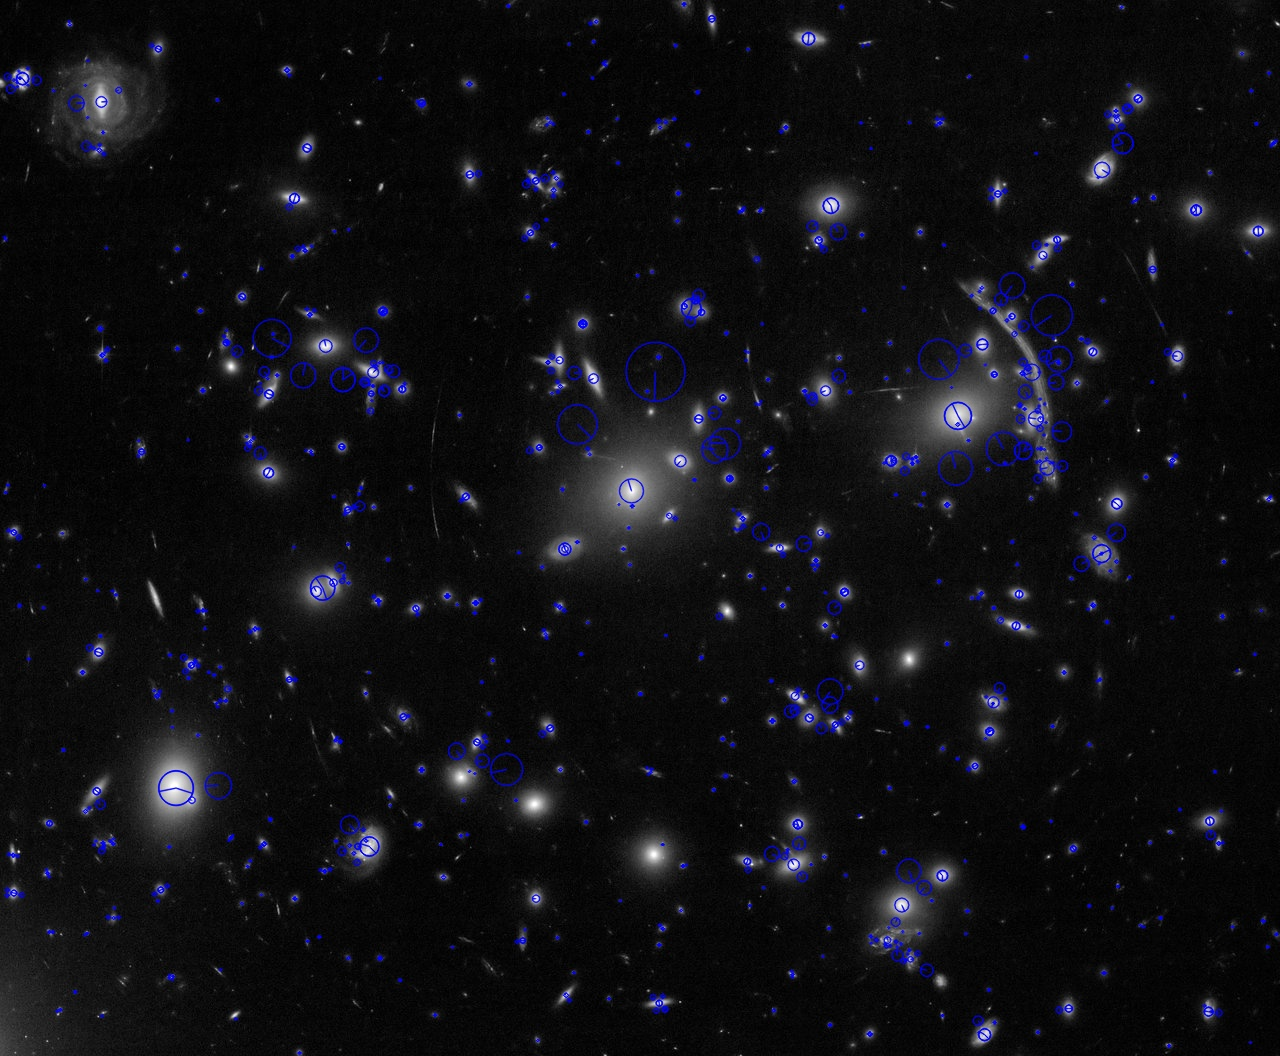
\includegraphics[width=0.85\textwidth]{sift_keypoints.jpg}
\caption{All detected SIFT keypoints (\texttt{sift\_keypoints.jpg}).}
\end{figure}

\textbf{b)} Color: \textbf{blue}, RGB $= (0, 0, 255)$. OpenCV uses BGR order, so in \texttt{cv2.drawKeypoints} I passed \texttt{color=(255, 0, 0)}, which puts the full value in the blue channel.

\textbf{c)} Number of SIFT keypoints: \textbf{1391}. Descriptor shape: \textbf{(1391, 128)}.

\textbf{d)} A keypoint is a distinctive point in the image (such as a bright blob or corner), with a location, scale, and orientation, that can be found again under changes such as scaling or rotation.

%--------------------------------------------------
\section{ORB Detection and Visualization}
\textbf{a)}
\begin{figure}[H]
\centering
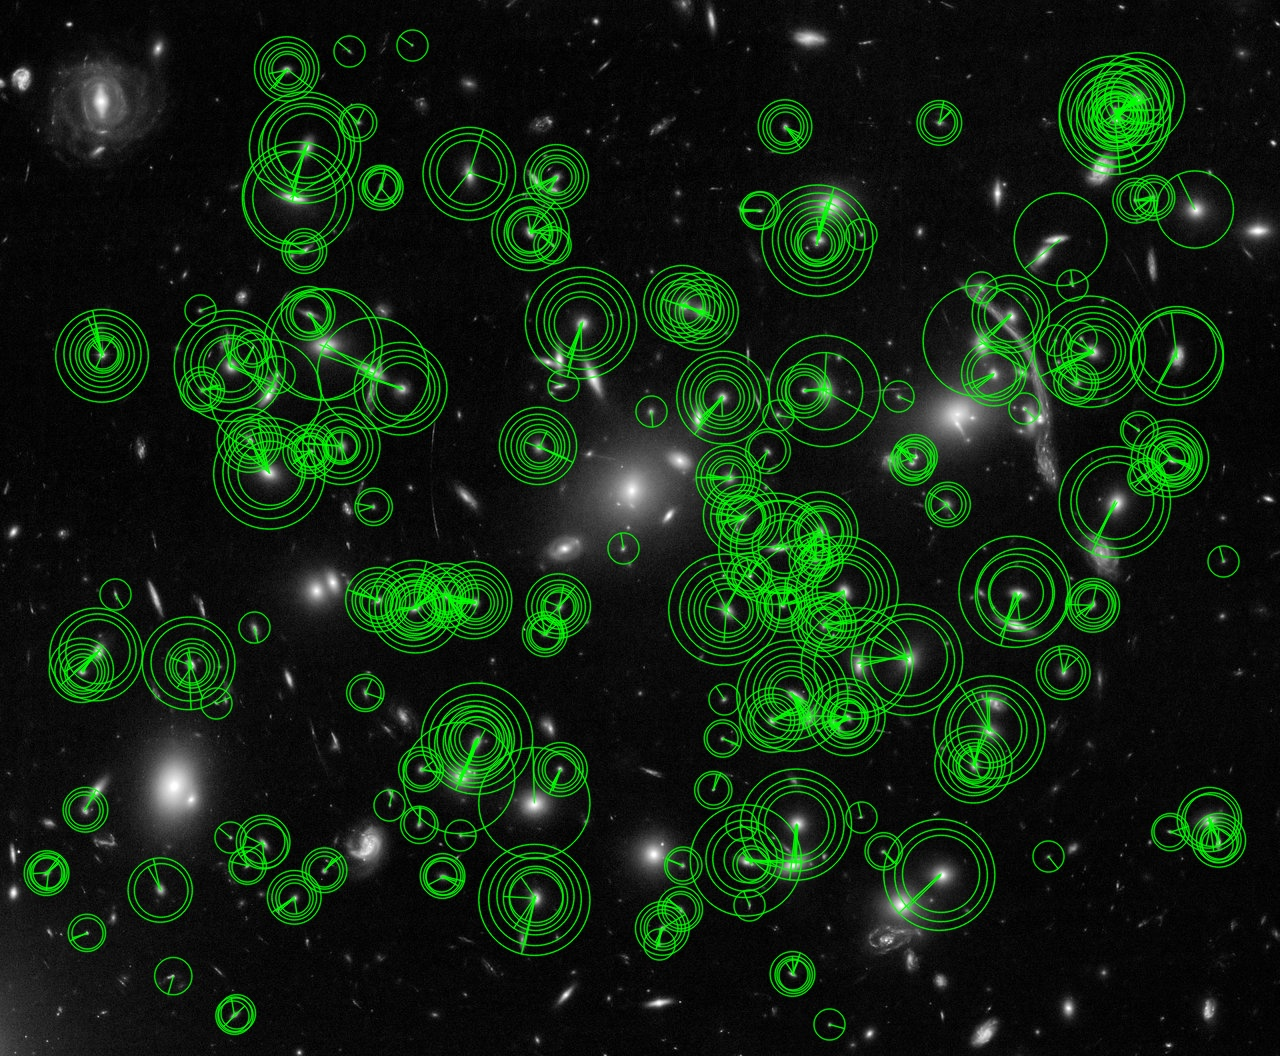
\includegraphics[width=0.85\textwidth]{orb_keypoints.jpg}
\caption{All detected ORB keypoints (\texttt{orb\_keypoints.jpg}).}
\end{figure}

\textbf{b)} Color: \textbf{green}, RGB $= (0, 255, 0)$. In BGR this is \texttt{(0, 255, 0)}, which I passed to \texttt{cv2.drawKeypoints}. Green has the same value in RGB and BGR.

\textbf{c)} Number of ORB keypoints: \textbf{500}. Descriptor shape: \textbf{(500, 32)}.

\textbf{d)} My final code uses \texttt{nfeatures=500}. I also tried other values:

\begin{center}
\begin{tabular}{|c|c|}
\hline
\texttt{nfeatures} & Keypoints detected \\ \hline
100  & 100 \\
500  & 500 \\
1000 & 1000 \\
2000 & 2000 \\ \hline
\end{tabular}
\end{center}

The number of detected points equals \texttt{nfeatures} each time, so it is the upper limit ORB keeps. By comparison, SIFT found 1391 keypoints with no limit set.

%--------------------------------------------------
\section{Strongest Keypoints}
\textbf{a)}
\begin{figure}[H]
\centering
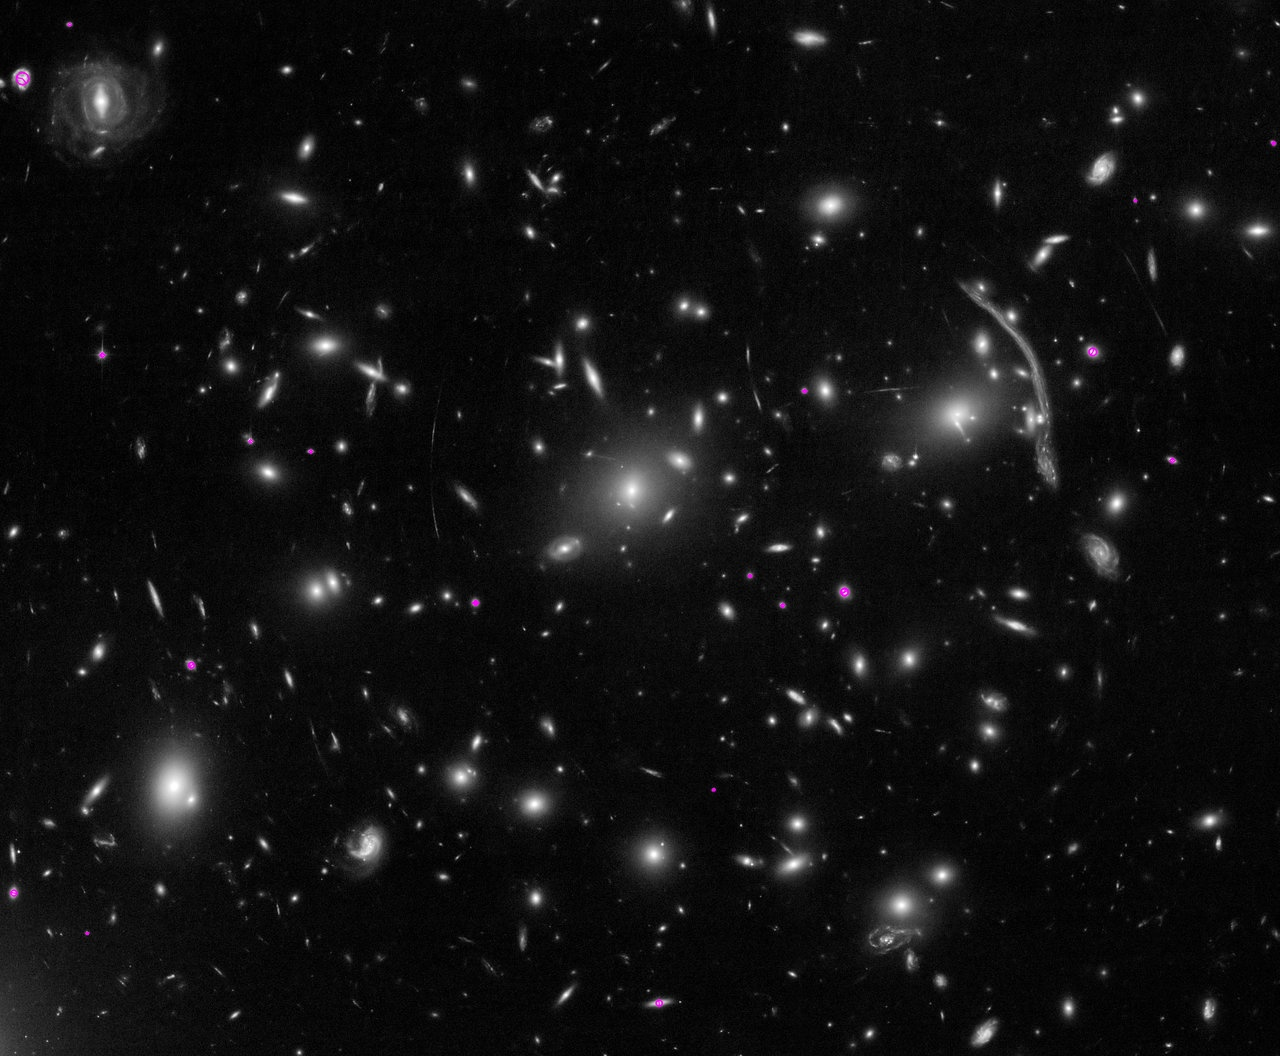
\includegraphics[width=0.7\textwidth]{sift_top50.jpg}
\caption{Top 50 strongest SIFT keypoints (\texttt{sift\_top50.jpg}), drawn in magenta.}
\end{figure}
\begin{figure}[H]
\centering
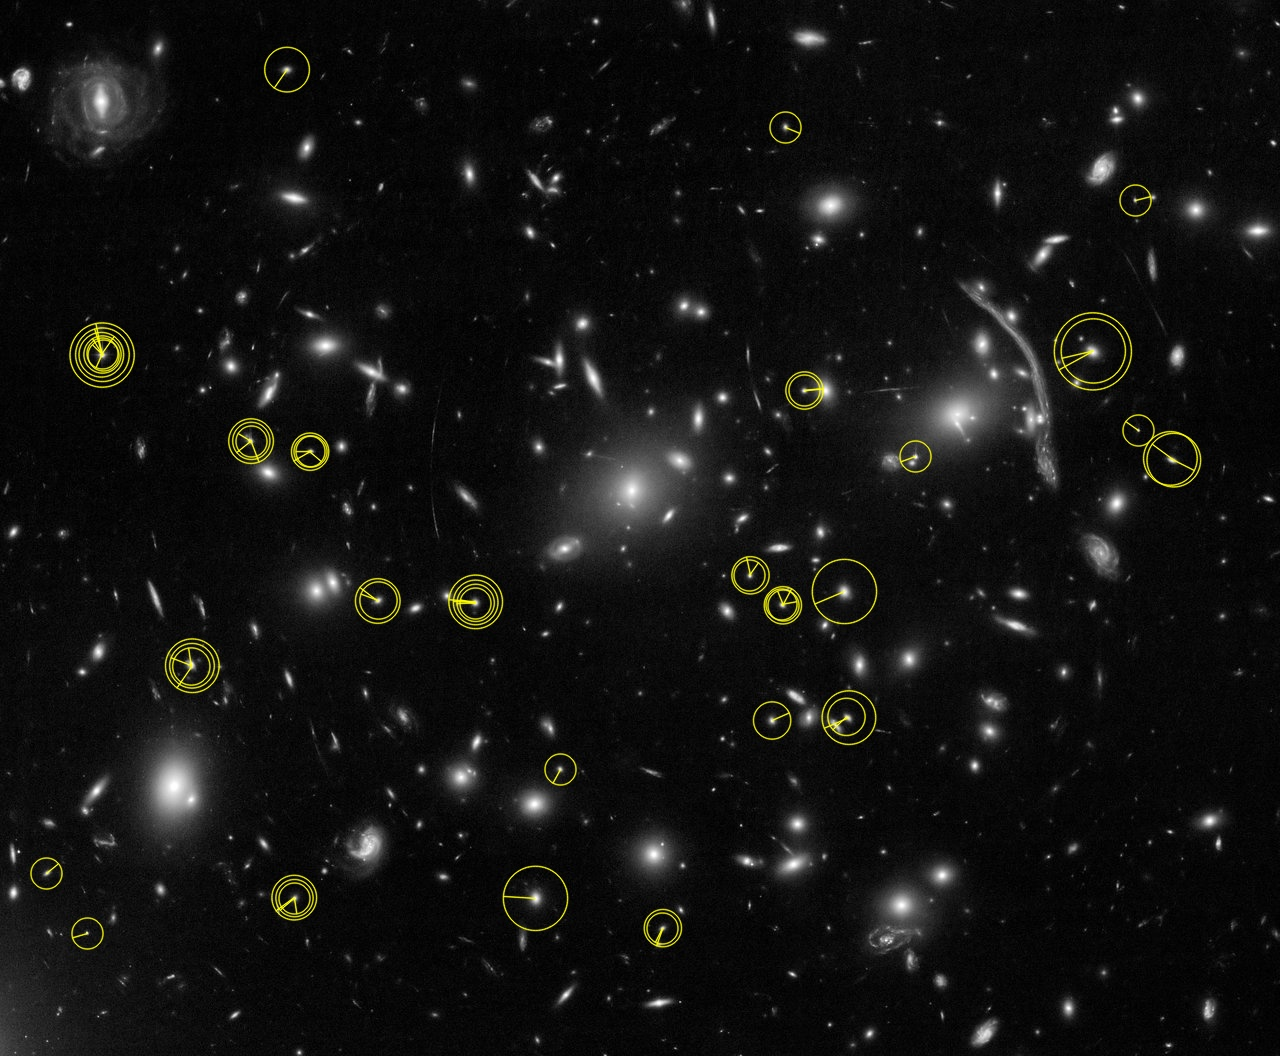
\includegraphics[width=0.7\textwidth]{orb_top50.jpg}
\caption{Top 50 strongest ORB keypoints (\texttt{orb\_top50.jpg}), drawn in yellow.}
\end{figure}

\textbf{b)} Response is a score of how strong or distinct a keypoint is, such as how clearly it stands out from its surroundings. A higher response means the detector is more confident that the point is a real feature. The keypoints were sorted by this value to get the top 50.

\textbf{c)} Strong keypoints are more stable and repeatable, so they are more likely to be found again in a second image. This gives fewer false matches and makes matching faster.

%--------------------------------------------------
\section{Descriptor Values}
\textbf{a)} First printed values (first 10 values of the first descriptor):
\begin{lstlisting}[numbers=none]
SIFT: [11.  2.  0.  0.  0.  1.  2. 10. 25. 13. ...]   (128 values, float)
ORB:  [ORB_VALUES_HERE ...]                          (32 values, integers)
\end{lstlisting}

\textbf{b)} A descriptor is a vector of numbers that describes the local image patch around a keypoint (for example the gradient directions or intensity comparisons). Two keypoints can be matched by comparing their descriptors.

\textbf{c)} SIFT descriptors have 128 elements and are floats (values here from 0 to 150). ORB descriptors have 32 elements and are 8-bit integers, with values from 0 to 255 (32 bytes, or 256 bits).

%--------------------------------------------------
\section{Descriptor Visualization}
\textbf{a)}
\begin{figure}[H]
\centering
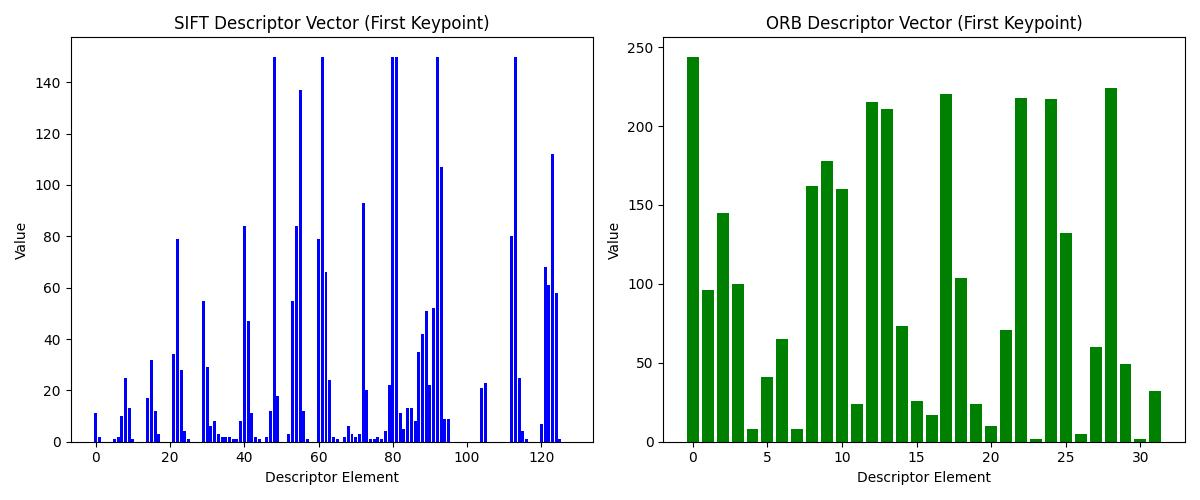
\includegraphics[width=\textwidth]{sift_descriptor_plot.jpg}
\caption{Descriptor vectors of the first keypoint (\texttt{sift\_descriptor\_plot.jpg}).}
\end{figure}

\textbf{b)} \texttt{plt.subplots} to create the figure and \texttt{axes.bar} (\texttt{matplotlib.pyplot.bar}) to draw the bars.

\textbf{c)} Each bar is one element of the descriptor vector of the first keypoint. The x-axis is the element index (0--127 for SIFT, 0--31 for ORB) and the height is that element's value. Many SIFT elements are close to zero with a few large ones, while the ORB bytes are spread over 0--255.

%--------------------------------------------------
\appendix
\section{Final Python Code}
\lstinputlisting{lab7sourcecode.py}

\end{document}
